\documentclass[12pt]{article}
\usepackage[left=1cm, right=1cm, top=2cm,bottom=1.5cm]{geometry} 

\usepackage[parfill]{parskip}
\usepackage[utf8]{inputenc}
\usepackage[T2A]{fontenc}
\usepackage[russian]{babel}
\usepackage{enumitem}
\usepackage[normalem]{ulem}
\usepackage{amsfonts, amsmath, amsthm, amssymb, mathtools,xcolor}
\usepackage{blkarray}

\usepackage{tabularx}
\usepackage{hhline}

\usepackage{accents}
\usepackage{fancyhdr}
\pagestyle{fancy}
\renewcommand{\headrulewidth}{1.5pt}
\renewcommand{\footrulewidth}{1pt}

\usepackage{graphicx}
\usepackage[figurename=Рис.]{caption}
\usepackage{subcaption}
\usepackage{float}

%%Наименование папки откуда забирать изображения
\graphicspath{ {./images/} }

%%Изменение формата для ввода доказательства
\renewcommand{\proofname}{$\square$  \nopunct}
\renewcommand\qedsymbol{$\blacksquare$}

%%Изменение отступа на таблицах
\addto\captionsrussian{%
	\renewcommand{\proofname}{$\square$ \nopunct}%
}
%% Римские цифры
\newcommand{\RN}[1]{%
	\textup{\uppercase\expandafter{\romannumeral#1}}%
}

%% Для удобства записи
\newcommand{\MR}{\mathbb{R}}
\newcommand{\MC}{\mathbb{C}}
\newcommand{\MQ}{\mathbb{Q}}
\newcommand{\MN}{\mathbb{N}}
\newcommand{\MZ}{\mathbb{Z}}
\newcommand{\MTB}{\mathbb{T}}
\newcommand{\MTI}{\mathbb{I}}
\newcommand{\MI}{\mathrm{I}}
\newcommand{\MCI}{\mathcal{I}}
\newcommand{\MJ}{\mathrm{J}}
\newcommand{\MH}{\mathrm{H}}
\newcommand{\MT}{\mathrm{T}}
\newcommand{\MU}{\mathcal{U}}
\newcommand{\MV}{\mathcal{V}}
\newcommand{\MB}{\mathcal{B}}
\newcommand{\MF}{\mathcal{F}}
\newcommand{\MW}{\mathcal{W}}
\newcommand{\ML}{\mathcal{L}}
\newcommand{\MP}{\mathcal{P}}
\newcommand{\VN}{\varnothing}
\newcommand{\VE}{\varepsilon}
\newcommand{\dx}{\, dx}
\newcommand{\dy}{\, dy}
\newcommand{\dz}{\, dz}
\newcommand{\dd}{\, d}


\theoremstyle{definition}
\newtheorem{defn}{Опр:}
\newtheorem{rem}{Rm:}
\newtheorem{prop}{Утв.}
\newtheorem{exrc}{Упр.}
\newtheorem{problem}{Задача}
\newtheorem{lemma}{Лемма}
\newtheorem{theorem}{Теорема}
\newtheorem{corollary}{Следствие}

\newenvironment{cusdefn}[1]
{\renewcommand\thedefn{#1}\defn}
{\enddefn}

\DeclareRobustCommand{\divby}{%
	\mathrel{\text{\vbox{\baselineskip.65ex\lineskiplimit0pt\hbox{.}\hbox{.}\hbox{.}}}}%
}
\DeclareRobustCommand{\ndivby}{\mkern-1mu\not\mathrel{\mkern4.5mu\divby}\mkern1mu}


%Короткий минус
\DeclareMathSymbol{\SMN}{\mathbin}{AMSa}{"39}
%Длинная шапка
\newcommand{\overbar}[1]{\mkern 1.5mu\overline{\mkern-1.5mu#1\mkern-1.5mu}\mkern 1.5mu}
%Функция знака
\DeclareMathOperator{\sgn}{sgn}

%Функция ранга
\DeclareMathOperator{\rk}{\text{rk}}
\DeclareMathOperator{\diam}{\text{diam}}


%Обозначение константы
\DeclareMathOperator{\const}{\text{const}}

\DeclareMathOperator{\codim}{\text{codim}}

\DeclareMathOperator*{\dsum}{\displaystyle\sum}
\newcommand{\ddsum}[2]{\displaystyle\sum\limits_{#1}^{#2}}

%Интеграл в большом формате
\DeclareMathOperator{\dint}{\displaystyle\int}
\newcommand{\ddint}[2]{\displaystyle\int\limits_{#1}^{#2}}
\newcommand{\ssum}[1]{\displaystyle \sum\limits_{n=1}^{\infty}{#1}_n}

\newcommand{\smallerrel}[1]{\mathrel{\mathpalette\smallerrelaux{#1}}}
\newcommand{\smallerrelaux}[2]{\raisebox{.1ex}{\scalebox{.75}{$#1#2$}}}

\newcommand{\smallin}{\smallerrel{\in}}
\newcommand{\smallnotin}{\smallerrel{\notin}}

\newcommand*{\medcap}{\mathbin{\scalebox{1.25}{\ensuremath{\cap}}}}%
\newcommand*{\medcup}{\mathbin{\scalebox{1.25}{\ensuremath{\cup}}}}%

\makeatletter
\newcommand{\vast}{\bBigg@{3.5}}
\newcommand{\Vast}{\bBigg@{5}}
\makeatother

%Промежуточное значение для sup\inf, поскольку они имеют разную высоту
\newcommand{\newsup}{\mathop{\smash{\mathrm{sup}}}}
\newcommand{\newinf}{\mathop{\mathrm{inf}\vphantom{\mathrm{sup}}}}

%Скалярное произведение
\newcommand{\inner}[2]{\left\langle #1, #2 \right\rangle }
\newcommand{\linsp}[1]{\left\langle #1 \right\rangle }
\newcommand{\linmer}[2]{\left\langle #1 \vert #2\right\rangle }

%Подпись символов снизу
\newcommand{\ubar}[1]{\underaccent{\bar}{#1}}

%% Шапка для букв сверху
\newcommand{\wte}[1]{\widetilde{#1}}
\newcommand{\wht}[1]{\widehat{#1}}
\newcommand{\ovl}[1]{\overline{#1}}

%%Трансформация Фурье
\newcommand{\fourt}[1]{\mathcal{F}\left(#1\right)}
\newcommand{\ifourt}[1]{\mathcal{F}^{-1}\left(#1\right)}

%%Символ вектора
\newcommand{\vecm}[1]{\overrightarrow{#1\,}}

%%Пространстов матриц
\newcommand{\matsq}[1]{\operatorname{Mat}_{#1}}
\newcommand{\mat}[2]{\operatorname{Mat}_{#1, #2}}

%Оператор для действ и мнимых чисел
\DeclareMathOperator{\IM}{\operatorname{Im}}
\DeclareMathOperator{\RE}{\operatorname{Re}}
\DeclareMathOperator{\li}{\operatorname{li}}
\DeclareMathOperator{\GL}{\operatorname{GL}}
\DeclareMathOperator{\SL}{\operatorname{SL}}
\DeclareMathOperator{\Char}{\operatorname{char}}
\DeclareMathOperator\Arg{Arg}

%Делимость чисел
\newcommand{\modn}[3]{#1 \equiv #2 \; (\bmod \; #3)}


%%Взятие в скобки, модули и норму
\newcommand{\parfit}[1]{\left( #1 \right)}
\newcommand{\modfit}[1]{\left| #1 \right|}
\newcommand{\sqparfit}[1]{\left\{ #1 \right\}}
\newcommand{\normfit}[1]{\left\| #1 \right\|}

%%Функция для обозначения равномерной сходимости по множеству
\newcommand{\uconv}[1]{\overset{#1}{\rightrightarrows}}
\newcommand{\uconvm}[2]{\overset{#1}{\underset{#2}{\rightrightarrows}}}


%%Функция для обозначения нижнего и верхнего интегралов
\def\upint{\mathchoice%
	{\mkern13mu\overline{\vphantom{\intop}\mkern7mu}\mkern-20mu}%
	{\mkern7mu\overline{\vphantom{\intop}\mkern7mu}\mkern-14mu}%
	{\mkern7mu\overline{\vphantom{\intop}\mkern7mu}\mkern-14mu}%
	{\mkern7mu\overline{\vphantom{\intop}\mkern7mu}\mkern-14mu}%
	\int}
\def\lowint{\mkern3mu\underline{\vphantom{\intop}\mkern7mu}\mkern-10mu\int}

%%След матрицы
\DeclareMathOperator*{\tr}{tr}

\makeatletter
\renewcommand*\env@matrix[1][*\c@MaxMatrixCols c]{%
	\hskip -\arraycolsep
	\let\@ifnextchar\new@ifnextchar
	\array{#1}}
\makeatother


%% Переопределение функции хи, чтобы выглядела более приятно
\makeatletter
\@ifdefinable\@latex@chi{\let\@latex@chi\chi}
\renewcommand*\chi{{\@latex@chi\smash[t]{\mathstrut}}} % want only bottom half of \mathstrut
\makeatletter

\setcounter{MaxMatrixCols}{20}

\begin{document}
\lhead{Аналитическая геометрия}
\chead{Пенской А.В.}
\rhead{Лекция - 1}
\section*{Введение}
В древней Греции изучались конический сечения Аполлонием Пергским. Он изучал, что будет если пересекать конус плоскостью. Какое получится множество точек? 

Из школьной геометрии можно показать, что если плоскость перпендикулярна оси конуса, то в сечении будет окружность. Но что будет при пересечении другими плоскостями, не обязательно ортогональными оси конуса? Оказывается, что ответ разный и изучать его тоже можно по-разному. 
\begin{figure}[H]
	\centering
	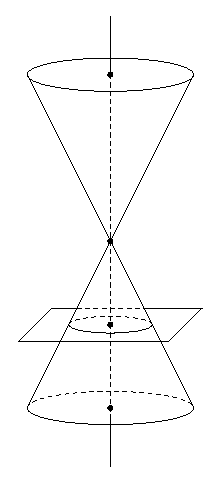
\includegraphics[width=0.20\textwidth]{ANGL1_1.eps}
	\caption{Сечение конуса, ортогонально его оси.}
	\label{1_1}
\end{figure}
Есть, например, \textbf{геометрическая теория}, которая близка к тому, что изучается в школе (синтетическая геометрия). Другой подход - \textbf{аналитический}. В своё время Декарт понял, что можно описывать точки в плоскости и в пространстве, приписывая им координаты. Более того, уже должно быть известно, что некоторые геометрические объекты удобно описывать уравнениями. 

\textbf{\uline{Аналитический подход}}: Изучение геометрических объектов, с помощью уравнений. 

Этот подход является более продуктивным, чем геометрический, поэтому мы немного поговорим про геометрический подход, а затем перейдем в аналитический.
\newpage
\section*{Геометрическая теория конических сечений}
\begin{defn}
	\uwave{Коническим сечением} или \uwave{коникой} называют секущую плоскость, которая не должна проходить через вершину конуса.
\end{defn}
\begin{rem}
	Отметим, что в аналитическом подходе из-за того, что коники описываются уравнениями второго порядка, они будут называтся квадриками. Но не все квадрики являются кониками. Есть уравнения второго порядка, которые описывают вовсе не конические сечения, например $xy = 0$ - описывает крест: $x = 0, \, y = 0$.
\end{rem}

\begin{defn}
	\uwave{Эллипсом} называется геометрическое место точек (то есть, множество), таких, что сумма расстояний от них до двух фиксированных точек (называемых \uwave{фокусами эллипса}) постоянна.
\end{defn}
Пусть $F_1, F_2$ - фокусы, $|xF_1| + |xF_2| = 2a$. Тогда эллипс будет иметь вид:
\begin{figure}[H]
	\centering
	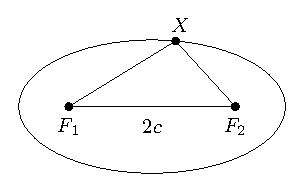
\includegraphics[width=0.3\textwidth]{ANGL1_2.eps}
	\caption{Эллипс.}
	\label{1_2}
\end{figure}
Расстояние между фокусами обычно обозначается через $2c$ и ради осмысленности множества накладывается условие $a > c$. Если $a = c \Rightarrow$ просто отрезок, если $a < c$, то получим пустое множество.
\begin{defn}
	\uwave{Гиперболой} называется геометрическое место точек - ГМТ, таких, что модуль разность расстояний до двух фиксированных точек (называемых \uwave{фокусами гипербол}) постоянен.
\end{defn}
Пусть $F_1, F_2$ - фокусы, $||xF_1| - |xF_2|| = 2a$. Тогда гипербола будет иметь вид:
\begin{figure}[H]
	\centering
	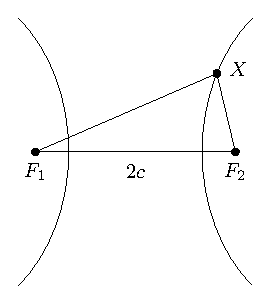
\includegraphics[width=0.2\textwidth]{ANGL1_3.eps}
	\caption{Гипербола.}
	\label{1_3}
\end{figure}
Расстояние между фокусами обычно обозначается через $2c$ и ради осмысленности множества накладывается условие $a < c$.
\begin{defn}
	\uwave{Параболой} называется ГМТ, равноудаленных от фиксированной точки (называемой \uwave{фокусом параболы}) и фиксированной прямой, называемой \uwave{директриссой}. 
\end{defn}
Пусть $F$ - фокус параболы, $d$ - директрисса, $\rho(x,d) = |XF|$. Тогда парабола будет иметь вид:
\begin{figure}[H]
	\centering
	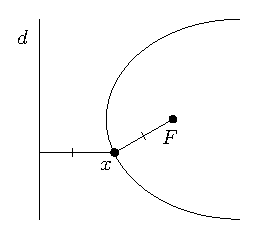
\includegraphics[width=0.25\textwidth]{ANGL1_4.eps}
	\caption{Парабола.}
	\label{1_4}
\end{figure}

Таким образом, у нас есть три типа разных кривых $\Rightarrow$ плоскость может пересекать круговой конус тремя принципиально разными способами. Рассмотрим эти способы.

\begin{enumerate}[label=\arabic*)]
	\item \uwave{Случай эллипса}: наклонная плоскость в пересечении с конусом даёт эллипс:
	\begin{figure}[H]
		\centering
		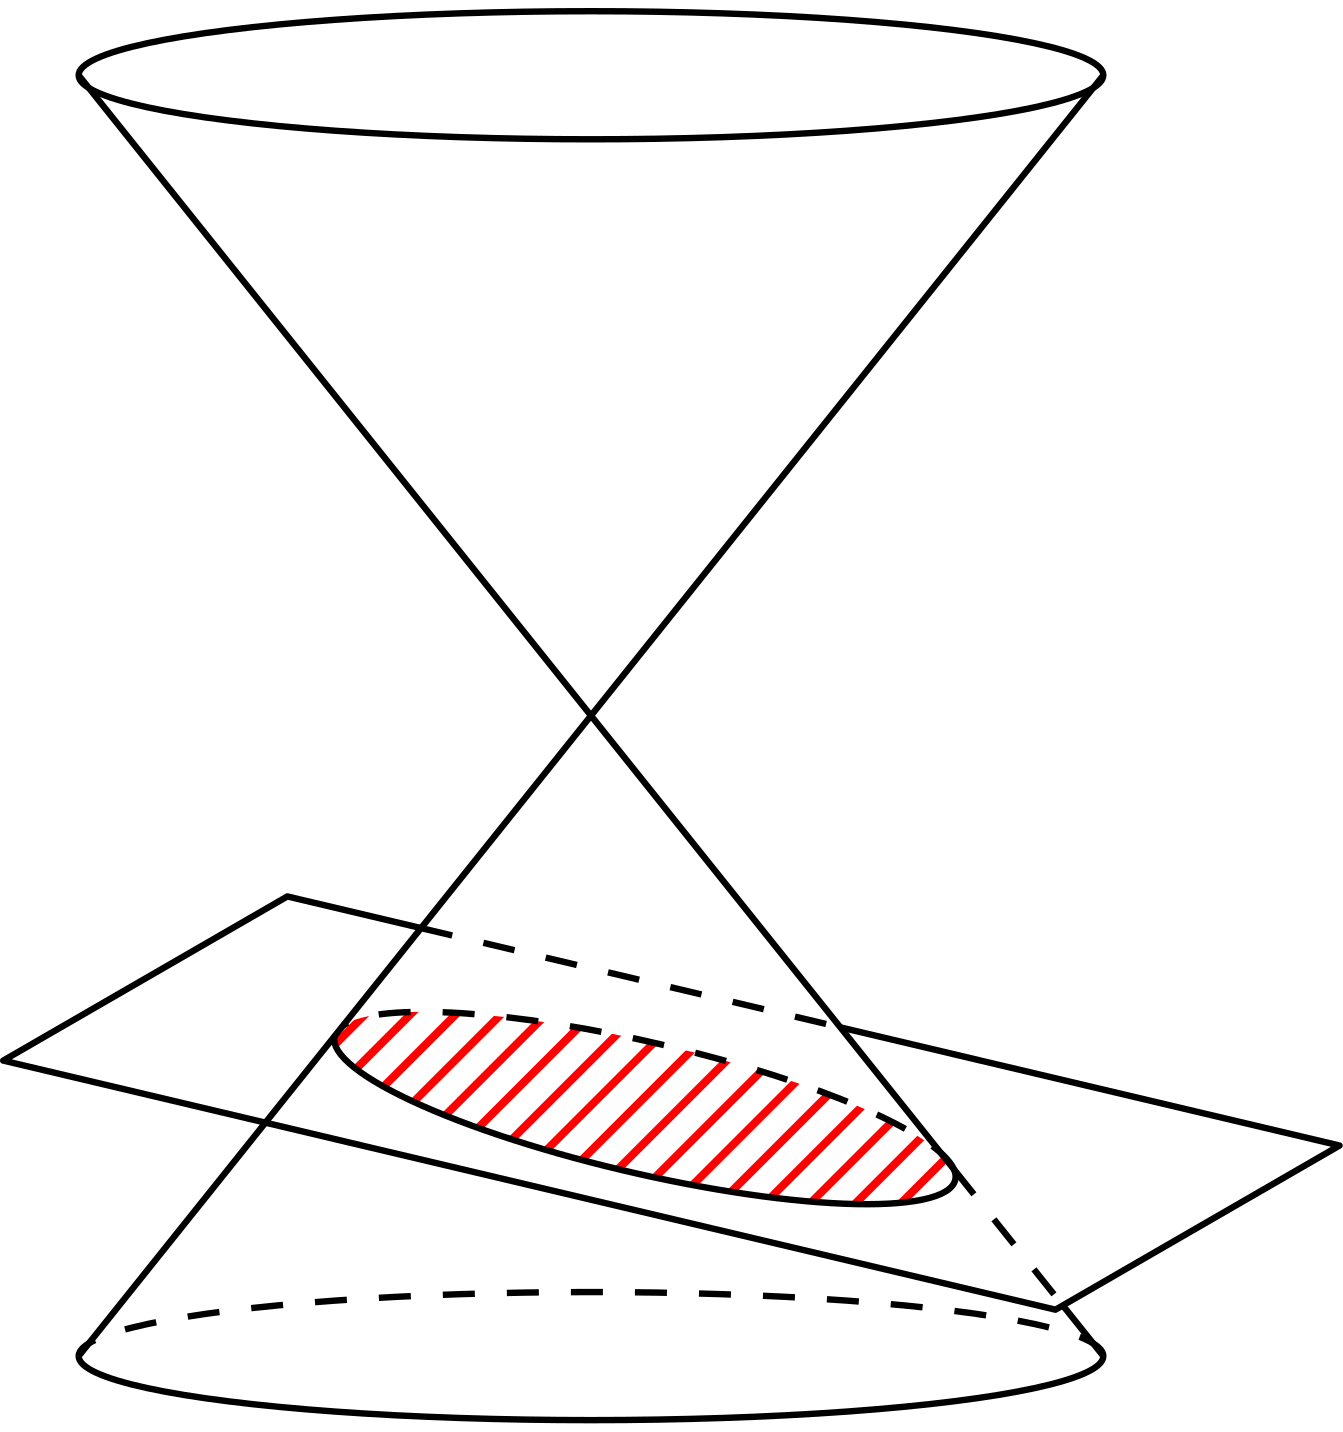
\includegraphics[width=0.25\textwidth]{ANGL1_5.png}
		\caption{Пересечение конуса плоскостью даёт эллипс.}
		\label{1_5}
	\end{figure}
	\item \uwave{Случай параболы}: наклонная плоскость в пересечении с конусом даёт параболу:
	\begin{figure}[H]
		\centering
		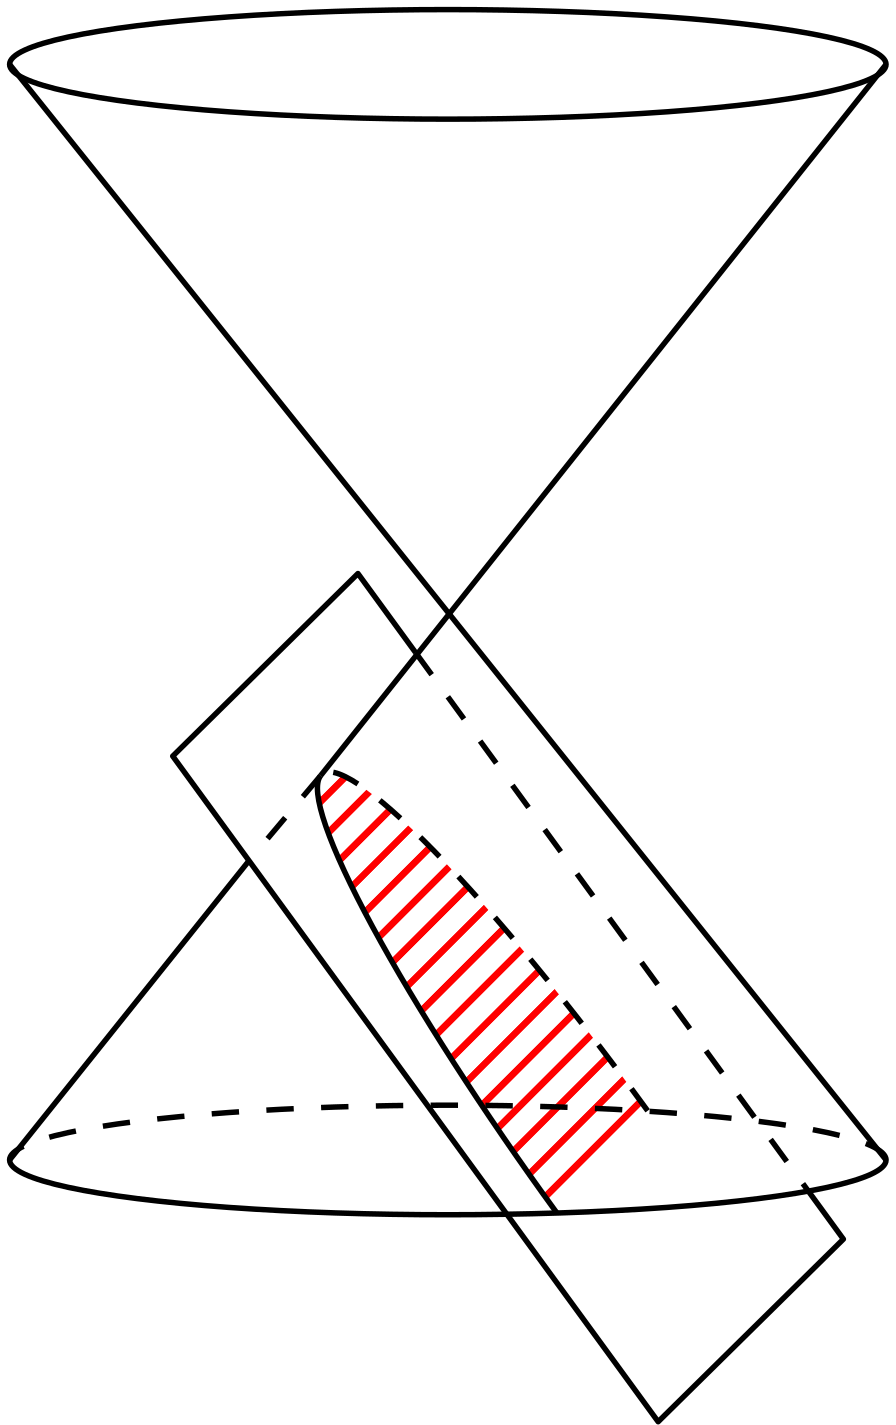
\includegraphics[width=0.2\textwidth]{ANGL1_6.png}
		\caption{Пересечение конуса плоскостью даёт параболу.}
		\label{1_6}
	\end{figure}
	\item \uwave{Случай гиперболы}: наклонная плоскость в пересечении с конусом даёт гиперболу:
	\begin{figure}[H]
		\centering
		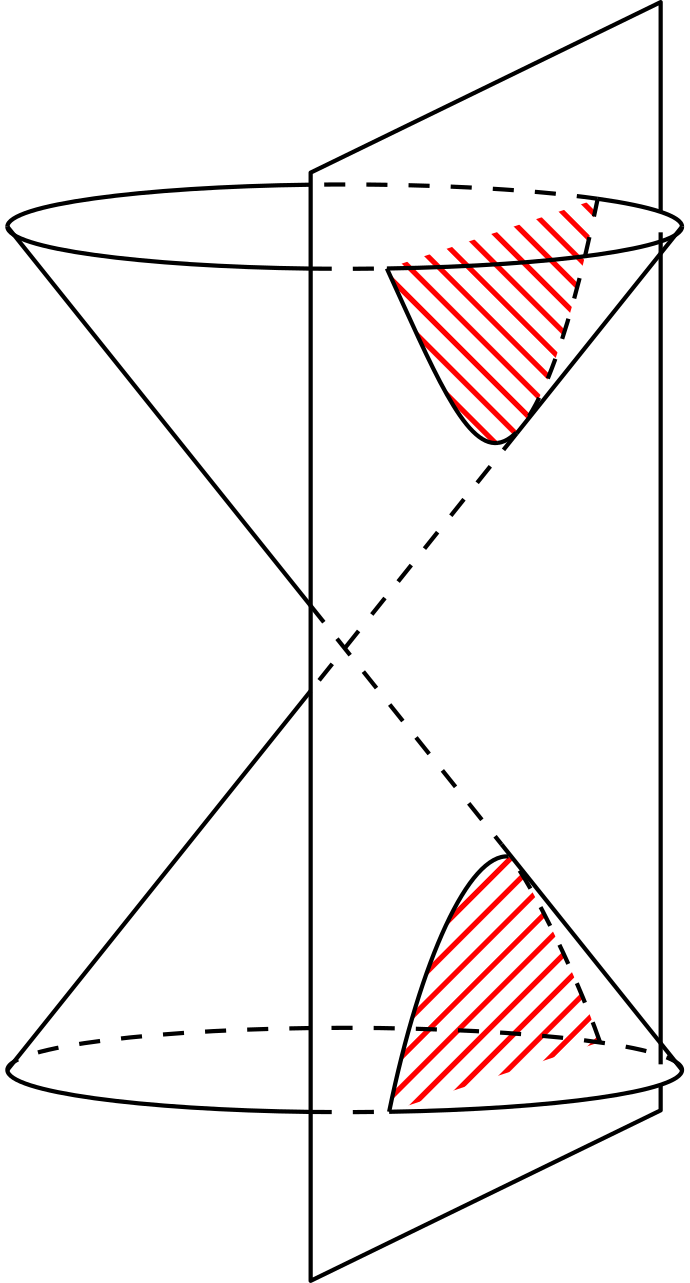
\includegraphics[width=0.2\textwidth]{ANGL1_7.png}
		\caption{Пересечение конуса плоскостью даёт гиперболу.}
		\label{1_7}
	\end{figure}
\end{enumerate}
Лучше всего это можно понять если нарисовать сечение плоскостью, ортогональной секущей плоскости и содержащей ось конуса.
\begin{figure}[H]
	\centering
	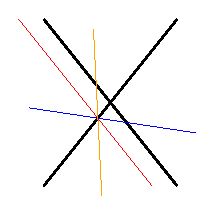
\includegraphics[width=0.25\textwidth]{ANGL1_8.eps}
	\caption{Сечение плоскостью, ортогональной секущей плоскости и содержащей ось конуса.}
	\label{1_8}
\end{figure}
На рисунке изображены прямые, проходящие через одну точку: 
\begin{enumerate}[label=\arabic*)]
	\item \textbf{конус} - жирные черные линии;
	\item \textbf{эллипс} - синяя линия;
	\item \textbf{парабола} - красная линия;
	\item \textbf{гипербола} - оранжевая линия;
\end{enumerate}
Как это можно доказать? В античности доказательства были достаточно сложные, мы же воспользуемся конструкцией под названием \uline{шары Данделена}. Покажем одно из доказательств в случае эллипса.
\begin{proof}
	Эллипс лежит в одной поле конуса, поэтому будем рассматривать её. Пусть $\pi$ - секущая плоскость. Впишем шар внутрь конуса, в самый низ. Пусть он касается нашей плоскости в точке $F_1$. В сечении это будет построение вписанной окружности. В сечении будет касание конуса в двух точках, в трехмерном пространстве это будет окружность на конусе. Затем впишем шар в конус, выше плоскости и будем уменьшать его радиус до тех пор, пока он не коснется плоскости $\pi$ с другой стороны, нежели предыдущий шар. Фактически, будем искать окружность, касающуюся трёх плоскостей. Она будет  касаться плоскости $\pi$ в точке $F_2$.
\end{proof}

\end{document}